%%%%%%%%%%%%%%%%%%%%%%%%%%%%%%%%%%%%%%%%%%%%%%%%%%
% Title page template been downloaded from:
% http://www.LaTeXTemplates.com
%%%%%%%%%%%%%%%%%%%%%%%%%%%%%%%%%%%%%%%%%%%%%%%%%%

\documentclass[a4paper]{article}
\RequirePackage[utf8]{inputenc}
\usepackage[portuguese]{babel}
\usepackage{listings}
\usepackage{color}
\usepackage{graphicx}
\usepackage{hyperref}
\usepackage{amsmath}
\usepackage{empheq}
\usepackage{framed}
\usepackage{float}
\usepackage{pdfpages}
\usepackage{graphicx}

\definecolor{dkgreen}{rgb}{0,0.6,0}
\definecolor{gray}{rgb}{0.5,0.5,0.5}
\definecolor{mauve}{rgb}{0.58,0,0.82}

\lstset{frame=tb,
  language=Java,
  aboveskip=3mm,
  belowskip=3mm,
  showstringspaces=false,
  columns=flexible,
  basicstyle={\small\ttfamily},
  numbers=none,
  numberstyle=\tiny\color{gray},
  keywordstyle=\color{blue},
  commentstyle=\color{dkgreen},
  stringstyle=\color{mauve},
  breaklines=true,
  breakatwhitespace=true,
  tabsize=3,
  literate=
  {á}{{\'a}}1 {é}{{\'e}}1 {í}{{\'i}}1 {ó}{{\'o}}1 {ú}{{\'u}}1
  {Á}{{\'A}}1 {É}{{\'E}}1 {Í}{{\'I}}1 {Ó}{{\'O}}1 {Ú}{{\'U}}1
  {à}{{\`a}}1 {è}{{\'e}}1 {ì}{{\`i}}1 {ò}{{\`o}}1 {ù}{{\`u}}1
  {À}{{\`A}}1 {È}{{\'E}}1 {Ì}{{\`I}}1 {Ò}{{\`O}}1 {Ù}{{\`U}}1
  {ä}{{\"a}}1 {ë}{{\"e}}1 {ï}{{\"i}}1 {ö}{{\"o}}1 {ü}{{\"u}}1
  {Ä}{{\"A}}1 {Ë}{{\"E}}1 {Ï}{{\"I}}1 {Ö}{{\"O}}1 {Ü}{{\"U}}1
  {â}{{\^a}}1 {ê}{{\^e}}1 {î}{{\^i}}1 {ô}{{\^o}}1 {û}{{\^u}}1
  {Â}{{\^A}}1 {Ê}{{\^E}}1 {Î}{{\^I}}1 {Ô}{{\^O}}1 {Û}{{\^U}}1
  {œ}{{\oe}}1 {Œ}{{\OE}}1 {æ}{{\ae}}1 {Æ}{{\AE}}1 {ß}{{\ss}}1
  {ç}{{\c c}}1 {Ç}{{\c C}}1 {ø}{{\o}}1 {å}{{\r a}}1 {Å}{{\r A}}1
  {€}{{\EUR}}1 {£}{{\pounds}}1
}

\newlength\dlf  % Define a new measure, dlf
\newcommand\alignedbox[2]{
% Argument #1 = before & if there were no box (lhs)
% Argument #2 = after & if there were no box (rhs)
&  % Alignment sign of the line
{
\settowidth\dlf{$\displaystyle #1$}  
    % The width of \dlf is the width of the lhs, with a displaystyle font
\addtolength\dlf{\fboxsep+\fboxrule}  
    % Add to it the distance to the box, and the width of the line of the box
\hspace{-\dlf}  
    % Move everything dlf units to the left, so that & #1 #2 is aligned under #1 & #2
\boxed{#1 #2}
    % Put a box around lhs and rhs
}
}

\newcommand{\HRule}{\rule{\linewidth}{0.5mm}} % Defines a new command for the horizontal lines, change thickness here

\begin{document}

\begin{titlepage}

\center % Center everything on the page
 
%----------------------------------------------------------------------------------------
%	HEADING SECTIONS
%----------------------------------------------------------------------------------------

\textsc{\LARGE Instituto Superior de Engenharia de Lisboa}\\[1.5cm] % Name of your university/college
\textsc{\Large Sistemas Distribuídos}\\[0.5cm] % Major heading such as course name

%----------------------------------------------------------------------------------------
%	TITLE SECTION
%----------------------------------------------------------------------------------------

\HRule \\[0.4cm]
{ \huge \bfseries Relatório da terceira série}\\[0.4cm] % Title of your document
\HRule \\[1.5cm]
 
%----------------------------------------------------------------------------------------
%	AUTHOR SECTION
%----------------------------------------------------------------------------------------

\begin{minipage}{0.4\textwidth}
\begin{flushleft} \large
\emph{Autoria:}\\
32632 Pedro \textsc{Pedroso} \\
33724 David \textsc{Raposo} \\
33404 Ricardo \textsc{Mata} \\
\end{flushleft}
\end{minipage}


%----------------------------------------------------------------------------------------
%	DATE SECTION
%----------------------------------------------------------------------------------------


\null
\vfill % Fill the rest of the page with whitespace
{\large \today}\\[3cm] % Date, change the \today to a set date if you want to be precise
\end{titlepage}

%----------------------------------------------------------------------------------------
%	ÍNDICE
%----------------------------------------------------------------------------------------

\newpage
\thispagestyle{empty} %Remove a númeração da página

\tableofcontents

%----------------------------------------------------------------------------------------
%	BODY
%----------------------------------------------------------------------------------------
\newpage
\setcounter{page}{1} %começa a contar as páginas apartir do 1

\section{Introdução}

Neste terceiro trabalho da disciplina de Sistemas Distribuídos, foi requerido que se implementasse as diferentes componentes de um sistema de pesquisa de automóveis e respetiva reserva.

Este sistema é composto pelos seguintes intervenientes:

\begin{itemize}

\item
\underline{Cliente}: Aplicação gráfica onde serão feitas as pesquisas e respetivos pedidos de reserva.

\item
\underline{Stands}: Aplicações que contêm um conjunto de carros, onde incidem as pesquisas e reservas dos clientes. Mantém dados persistentes usando ficheiros \emph{XML} para obter/guardar a informação necessária. 

\item
\underline{Broker}: Aplicação que o cliente comunicará para fazer a sua pesquisa e onde os \emph{stands} se podem registar para mais tarde ser propagada as pesquisas dos clientes.

\end{itemize}

\newpage

\section{Arquitetura}

\begin{figure}[H]
\centering
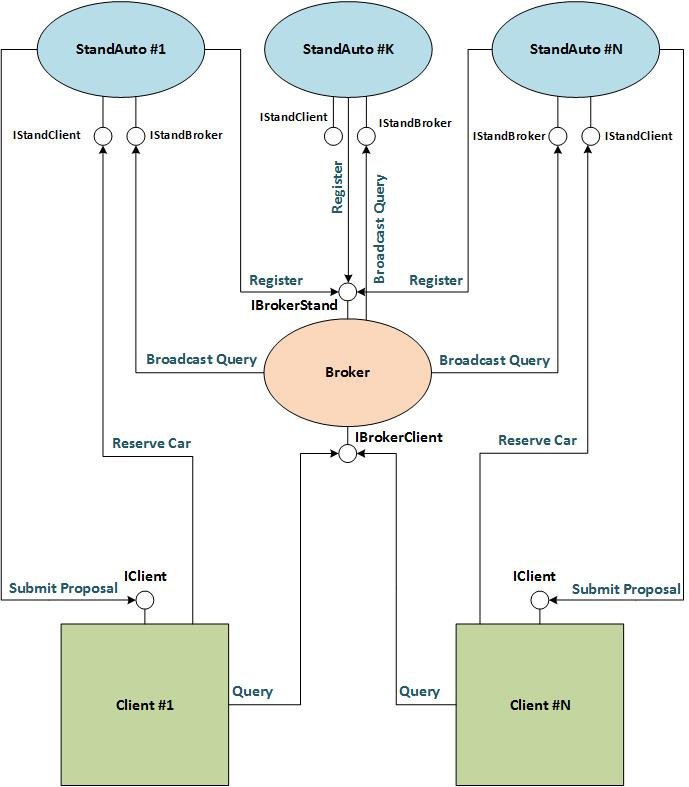
\includegraphics[width=100mm]{Arquitectura.jpg}
\caption{Arquitetura}
  \label{fig:httpHeaderReq}
\end{figure}

----------------------------------------------------------------------------------------------

As diversas aplicações foram desenvolvidas em \emph{c\#}. Na componente gráfica do cliente foi usado \emph{Windows Forms}, enquanto para a componente \emph{web} das diversas aplicações foi usado \emph{WCF}.

Para o desenvolvimento dos serviços, existem restrições em relação aos \emph{bindings} que podem ser usados (\emph{Binding wsHttpBinding} e \emph{basicHttpBinding}). Tendo em conta que não foi possível usar \emph{bindings} com suporte para \emph{callbacks}, optou-se por passar os endereços durante as diversas comunicações, para executar posteriormente a entrega/aceitação de propostas.

\newpage

\section{Componentes}

\subsection{\emph{Broker} } Componente intermédio para fazer \emph{broadcast} ás pesquisas dos clientes para os stands e para registar os mesmos.

\subsubsection{Serviços disponibilizados}
\begin{itemize} 

\item
\emph{\underline{IBrokerClient:}}
Serviço que permite aos clientes submeterem as suas pesquisas ao \emph{Broker}.
	\begin{itemize}
		\item
		Modo de instanciação: \underline{Singleton}\\
		Visto não haver alterações de objetos neste serviço e admitindo que haverá vários clientes a fazer várias pesquisas então não seria razoável criar um objeto por chamada. Um só objeto consegue lidar com os pedidos de forma eficaz.
		\item
		Modo de controlo de concorrência: \underline{Multiple}\\
		Ao receber vários pedidos será razoável que o processamento desses pedidos seja \emph{multi-thread}. Visto não haver alterações nenhumas em variáveis no \emph{Singleton} então não é necessário sincronismo adicional por parte do \emph{Broker}.
		\item
		Binding utilizado: \underline{basicHttpBinding}\\
		Visto a informação enviada para o \emph{Broker} não ter dados importantes, é utilizado \emph{basicHttpBinding} para simplificar a mensagem enviada. Visto também que o cliente não obtém \emph{feedback} nesta comunicação, os métodos estão declarados como \emph{IsOneWay}. Esta opção faz com que o \emph{binding} seja imediatamente libertado após a receção da mensagem por parte do \emph{Broker} e liberta este \emph{binding} para ser utilizado pelos stands para submissão de propostas.
	\end{itemize}
\item
\emph{\underline{IBrokerStand:}}
Serviço que permite que um \emph{stand} se registe no \emph{Broker} para receber as pesquisas dos clientes.
		\begin{itemize}
		\item
		Modo de instanciação: \underline{Singleton}\\
		Devido a existência de dois serviços, foi necessário usar \emph{partial classes}, logo, o modo de instanciação teria de ser igual a \emph{IBrokerClientService}.
		\item
		Modo de controlo de concorrência: \underline{Multiple}\\
		Com a possibilidade de vários stands se registarem ao mesmo tempo, utilizamos um modo de concorrência \emph{Multiple}. Isto cria problemas em relação ao sincronismo do objeto que está a ser usado para guardar o registo dos \emph{stands}, em que se optou por usar mecanismos de \emph{lock} que, visto o registo de \emph{stands} ser algo que ocorrerá ocasionalmente, não vai afetar a \emph{performance} por ser um mecanismo bloqueante.
		
		\item
		Binding utilizado: \underline{wsHttpBinding}\\
		Binding utilizado como requisito não funcional.
	\end{itemize}
\end{itemize}

\newpage


\subsection{\emph{Client}}
Componente que faz a submissão das propostas e reserva dos carros. O cliente tem uma interface gráfica para melhor ajudar a visualização das propostas e submissão das várias pesquisas.
\subsubsection{Serviços disponibilizados}
\begin{itemize} 

\item
\emph{\underline{IClient:}}
Serviço que permite aos stands submeteram as propostas aos clientes.
	\begin{itemize}
		\item
		Modo de instanciação: \underline{PerCall}\\
		Um cliente só receberá propostas depois de efetuar uma pesquisa. Isto faz com que usar um objeto \emph{Singleton} não seja razoável no sentido que não há necessidade de manter um objeto de serviço alocado quando não se espera mais propostas. Por esta razão foi escolhido o método de instanciação \emph{PerCall} que cria um objeto de serviço que tem a duração da submissão da proposta.
		\item
		Modo de controlo de concorrência: \underline{Multiple}\\
		Para resolver os problemas de concorrência causados pelo controlo \emph{multiple} utilizamos o método \emph{beginInvoke} para obrigar a que as alterações à \emph{listbox} sejam feitas sempre na \emph{UI thread}.
		
		\item
		Binding utilizado: \underline{basicHttpBinding}\\
		Binding utilizado como requisito não funcional.
	\end{itemize}
\end{itemize}


\subsection{\emph{StandAuto}}
Componente que mantém persistente dados de carros e submete as propostas aos clientes com base nas pesquisas feitas.
\subsubsection{Serviços disponibilizados}
\begin{itemize} 

\item
\emph{\underline{IStandBroker:}}
Serviço que permite ao \emph{Broker} propagar a pesquisa aos \emph{stands}.
	\begin{itemize}
		\item
		Modo de instanciação: \underline{Singleton}\\
		Admitindo que este serviço irá estar frequentemente a receber pedidos vindos do \emph{Broker} é razoável a utilização de um objeto de serviço \emph{Singleton}.
		\item
		Modo de controlo de concorrência: \underline{Multiple}\\
		Vários pedidos implicam um ambiente \emph{multi-thread} portanto é usado o controlo de concorrência \emph{multiple}.
		Não é alterado nenhum objeto no \emph{stand} portanto não é necessário controlo de concorrência adicional.
		\item
		Binding utilizado: \underline{wsHttpBinding}\\
		Binding utilizado como requisito não funcional.
	\end{itemize}
	
	\item
\emph{\underline{IStandClient:}}
Serviço que permite aos clientes fazerem as suas reservas de carros.
	\begin{itemize}
		\item
		Modo de instanciação: \underline{Singleton}\\
		Admitindo que este serviço irá estar frequentemente a receber reservas vindos dos clientes é razoável a utilização de um objeto de serviço \emph{Singleton}.
		\item
		Modo de controlo de concorrência: \underline{Multiple}\\
		Várias reservas implicam um ambiente \emph{multi-thread} portanto é usado o controlo de concorrência \emph{multiple}. Visto haver mudança em variáveis (alterar o estado do carro para reservado) foi necessário implementar um mecanismo adicional de concorrência. Por isso utilizamos o mecanismo \emph{Interlocked.CompareExchange} para fazer a mudança de forma \emph{thread-safe}.
		\item
		Binding utilizado: \underline{wsHttpBinding}\\
		Binding utilizado como requisito não funcional.
	\end{itemize}
	
\end{itemize}


\subsubsection{Persistência de dados}

Um dos requisitos da aplicação, era que os carros que cada \emph{stand} disponibiliza, fossem persistentes através do uso de ficheiros \emph{.xml}. 

Como tal, definiu-se que cada carro teria a seguintes estrutura:

\begin{figure}[H]
	\begin{framed}
		\texttt{<car> \\
					\hspace*{5mm}<id> identificador dentro do \emph{stand} em concreto</id> \\
					\hspace*{5mm}<price> preço </price>\\
					\hspace*{5mm}<brand> marca </brand>\\
					\hspace*{5mm}<yearRegistration> ano do registo de matricula</yearRegistration>\\
					\hspace*{5mm}<isAvailable> Se está reservado de momento</isAvailable>\\
			    </car>
		}		
	\end{framed}
	\caption{Estrutura de cada entrada}
  \label{fig:httpHeaderReq}
\end{figure}

Não foi adicionado nenhum mecanismo de verificação da validade destes ficheiros (\emph{.xsd}), sendo apenas possível passar de não reservado para reservado. Qualquer outra alteração terá de ser feita manualmente sobre estes ficheiros.
Em relação a problemas gerados devido a concorrência, optou-se por assegurar apenas que não é possível múltiplas reservas no mesmo carro, informando o cliente desta situação.

\newpage

\section{Pesquisas}
Foram implementadas três tipos de pesquisas que o cliente pode usar para procurar pelos carros.

\begin{itemize}

\item
\underline{Por marca}\\
Retorna todos os carros da marca escolhida.

\item
\underline{Por ano}\\
Retorna todos os carros que tenham data de criação igual ou superior à data escolhida.

\item
\underline{Por preço}\\
Retorna todos os carros que tenham um preço menos ou igual ao preço escolhido.
\end{itemize}

\section{Tratamento de erros}
Para lidar com erros que poderão eventualmente acontecer utilizamos \emph{FaultContracts}.
No momento da reserva de um carro, se o carro já estiver reservado então lançamos uma exceção nossa \emph{AlreadyReservedFault} para dizer ao cliente que o carro já foi reservado sem ser necessário a criação de mais um \emph{binding} de comunicação.

\section{Ficheiros de configuração}
Cada componente está suportado por um ficheiro de configuração (\emph{app.config}) onde são definidos os \emph{endpoints} dos serviços disponibilizados assim como os \emph{endpoints} dos serviços dos outros componentes assim como todas as configuração associadas aos mesmos (tipos de \emph{binding}, contractos, etc). Assim é fácil mudar os \emph{endpoints} sem ser necessário o compilador.


\end{document}